\chapter{Analisis}
\label{ch:analisis}

Bab ini akan membahas analisis-analisis yang dilakukan dalam pengembangan perangkat lunak. Pada bab ini akan terdapat dua subbab utama, yang pertama, yaitu analisis perangkat lunak serupa yang saat ini sudah ada. Kemudian yang kedua, yaitu analisis sistem yang akan dikembangkan. 

\section{Analisis Perangkat Lunak Sejenis}
    Pembelajaran anatomi manusia saat ini telah tersedia melalui berbagai aplikasi lintas \textit{platform}, baik berbasis Windows, macOS, Android, maupun iOS, yang dikembangkan untuk mendukung proses pembelajaran anatomi manusia menggunakan pemodelan tiga dimensi (3D). Pada penelitian ini akan dilakukan analisis terhadap dua aplikasi yang dijadikan sebagai referensi utama, yaitu \textit{Anatomy 3D Atlas} dan \textit{Anatomy Learning} oleh Dr. Blanco.

   
     \subsection{\textit{Anatomy Learning}\footnote{Dr. Blanco, \textit{Anatomy Learning}, diunduh dari \url{https://play.google.com/store/apps/details?id=com.AnatomyLearning.Anatomy3DViewer3&hl=en} pada 10 Maret 2026, versi 3.1.5.}}
     
       \textit{Anatomy Learning} yang dikembangkan oleh\textit{ Med SoftWork for 3DMedical OÜ} merupakan \textit{platform} visualisasi anatomi berbasis \textit{real-time} 3D yang mendukung aksesibilitas lintas \textit{platform}. Sumber visual yang digunakan dalam aplikasi ini terdiri dari ribuan model anatomis yang telah dioptimasi guna menyajikan detail tubuh manusia yang presisi namun tetap responsif. 
       
       Aplikasi ini mengunggulkan fungsionalitas, mulai dari sistem identifikasi struktur pada atlas anatomi hingga fitur pemotongan virtual melalui kontrol transparansi lapisan tubuh. Selain itu, modul evaluasi mandiri (\textit{quizzes}) yang mendetail serta animasi gerakan dinamis anggota tubuh memberikan pengalaman belajar yang mendalam, di mana pengguna dapat memahami keterkaitan antara struktur tulang, sendi, otot dan organ dengan mekanisme pergerakan tubuh manusia secara fungsional.
        

        Berikut adalah fitur-fitur yang terdapat pada \textit{Anatomy Learning}:
    
         \begin{enumerate}
    		\item \textit{Atlas Anatomy}
            
                Fitur utama pada aplikasi ini adalah atlas anatomi di mana anatomi manusia diklasifikasikan ke dalam beberapa kategori utama, yang kemudian dibagi menjadi sub-kategori lebih spesifik:
                \begin{itemize}
                    \item \textit{Bones; Skeletal System }(Sistem Tulang)
                        \begin{itemize}
                            \item \textit{Head and Neck}.
                            \item \textit{Trunk}.
                            \item \textit{Upper Limb}.
                            \item \textit{Lower Limb}.
                        \end{itemize}
                    \item \textit{Joints; Articular System} (Sistem Sendi)
                        \begin{itemize}
                            \item \textit{Head and Neck}.
                            \item \textit{Trunk}.
                            \item \textit{Upper Limb}.
                            \item \textit{Lower Limb}.
                        \end{itemize}
                    \item {\textit{Muscles} (Sistem Otot)}
                        \begin{itemize}
                            \item \textit{Head and Neck}.
                            \item \textit{Trunk}.
                            \item \textit{Upper Limb}.
                            \item \textit{Lower Limb}.
                        \end{itemize}
                    \item serta berbagai kategori tambahan yang mencakup representasi fungsional dari berbagai organ, pembuluh, saraf, hingga perbedaan yang dimiliki setiap kelamin pada tubuh manusia.
                 \end{itemize}
                      \begin{figure}[H] 
                        \centering  
                        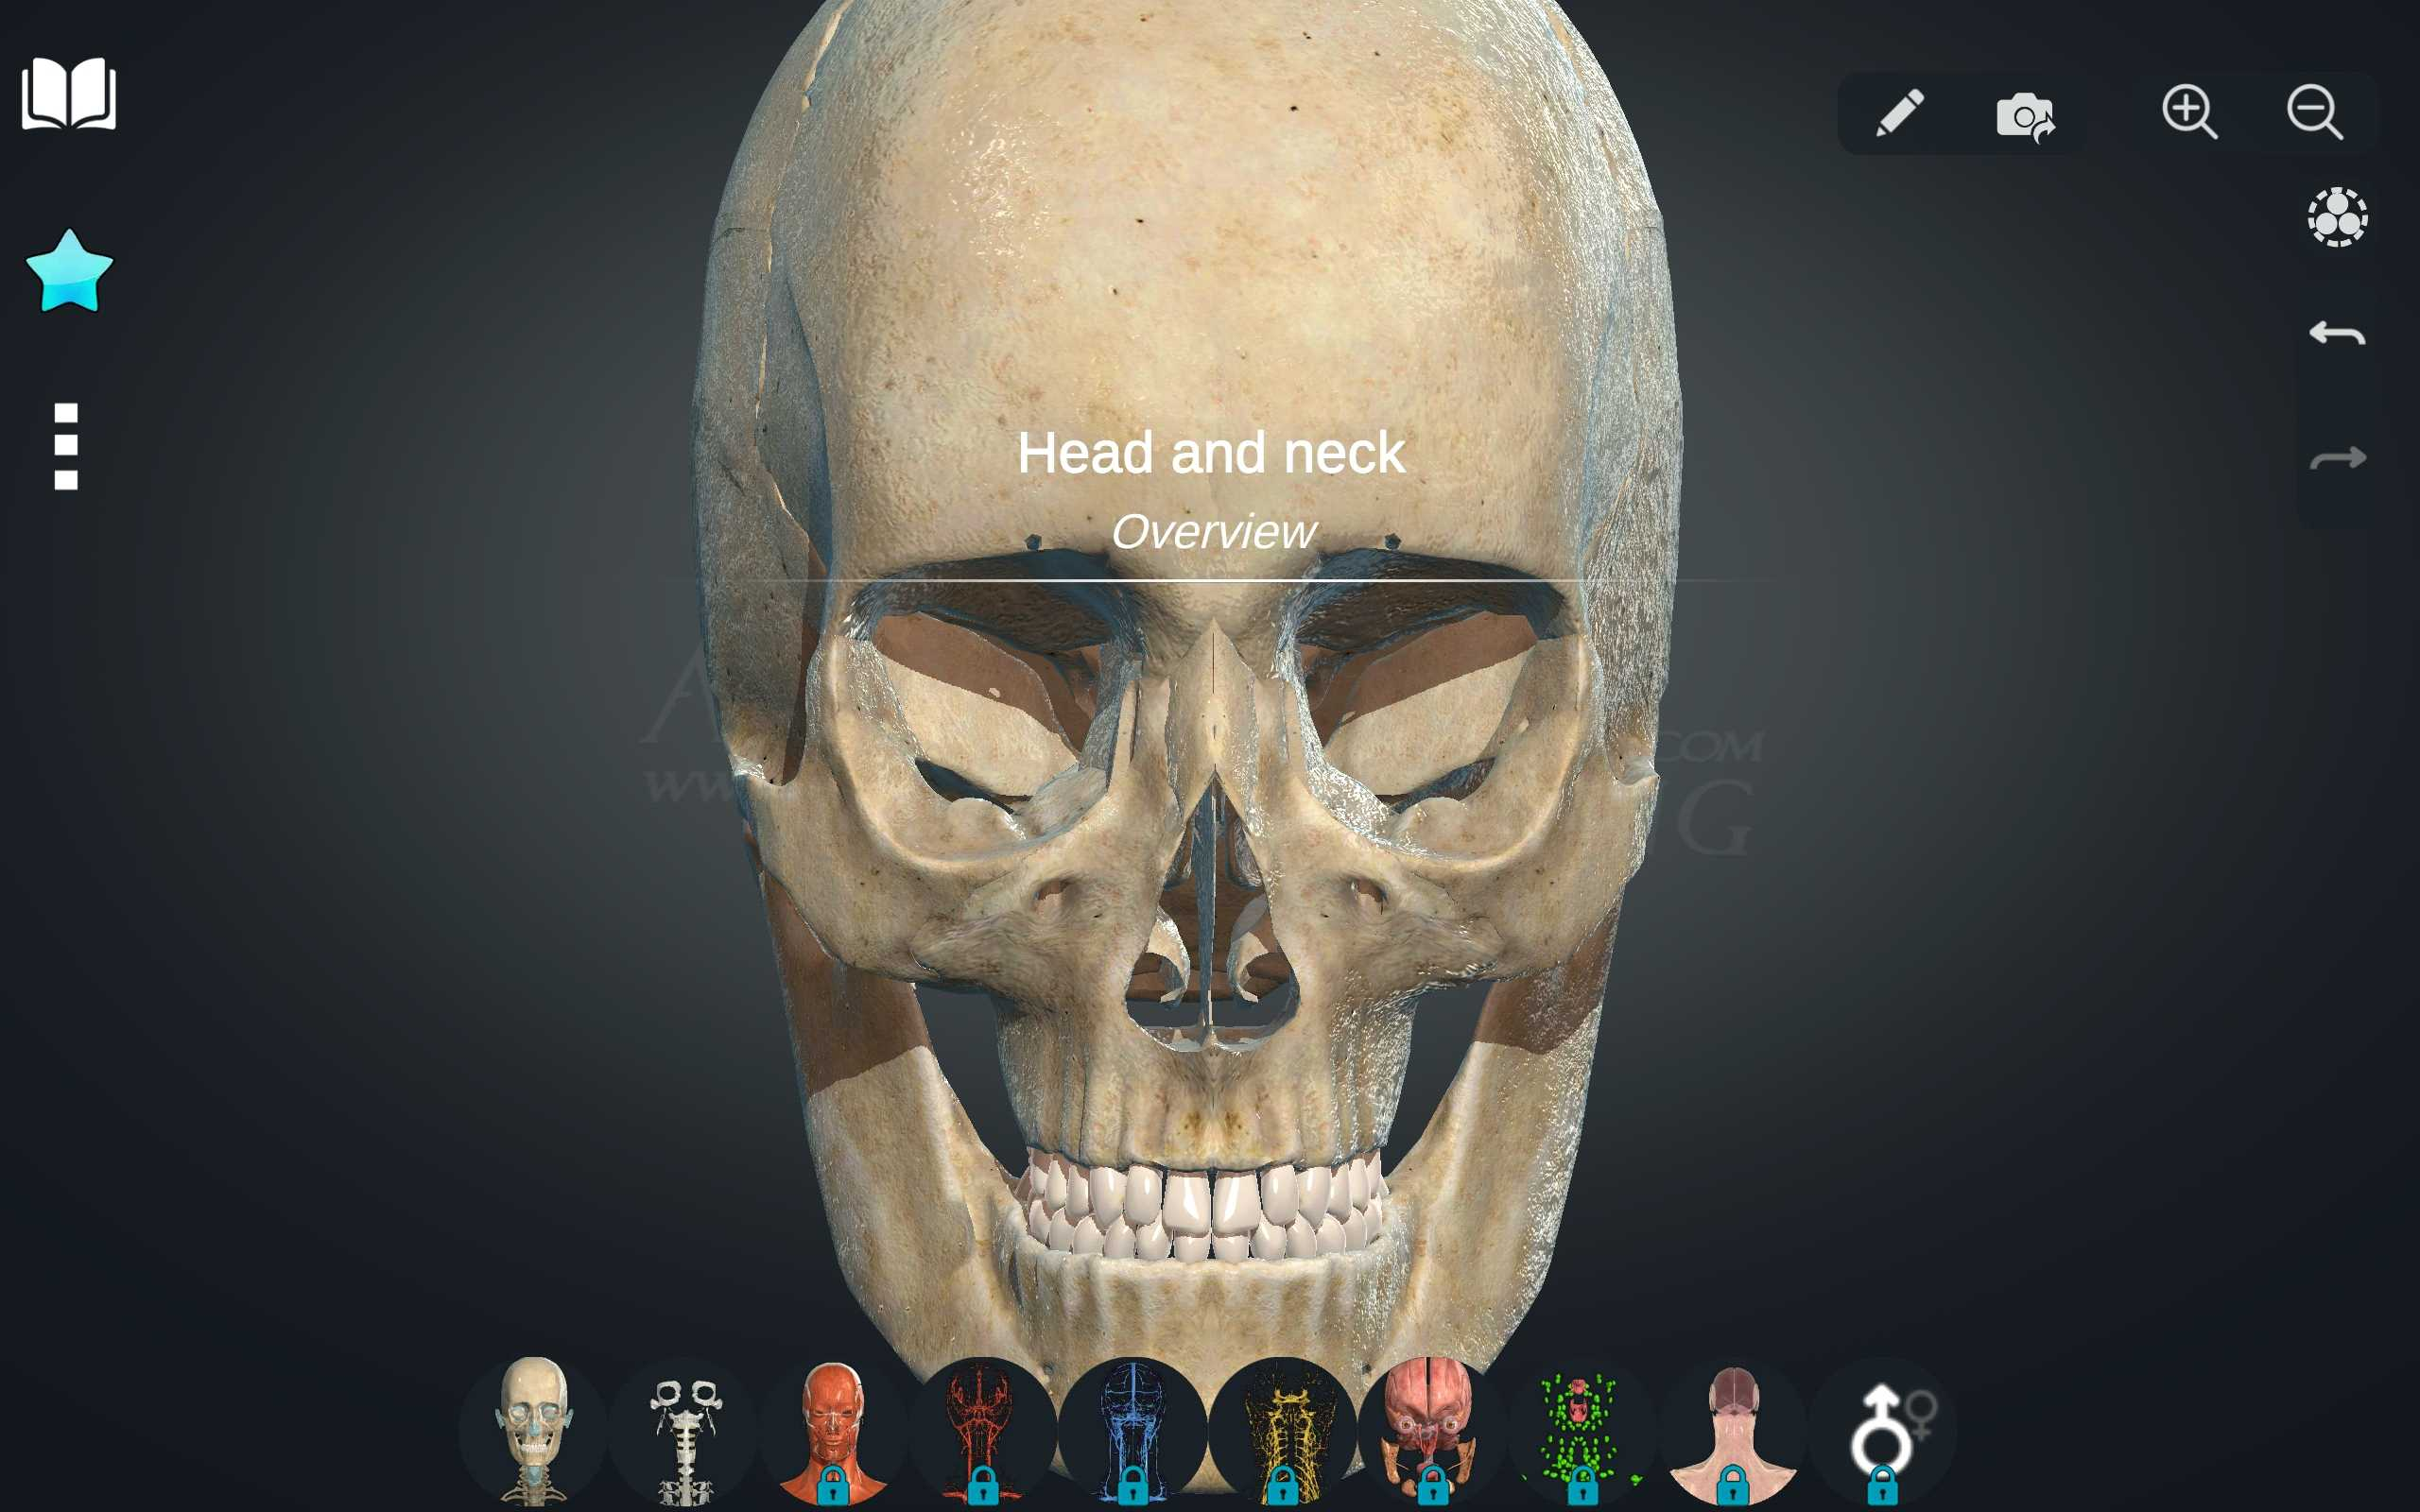
\includegraphics[width=0.8\textwidth]{Gambar/AnatomyLearning_AtlasAnatomyPreview.jpg}  
                        \caption [Halaman preview \textit{Atlas Anatomy} pada aplikasi \textit{Anatomy Learning}] {Halaman preview \textit{Atlas Anatomy} pada aplikasi \textit{Anatomy Learning}}  
                        \label{fig:PreviewAtlasAnatomyPage} 
                    \end{figure}
            \item {Quizzes}
            
                Fitur ini menyediakan modul soal bagi pengguna dengan klasifikasi yang lebih mendalam dibandingkan fitur Atlas Anatomy. Sebagai contoh, pada kategori sistem \textit{skeletal regio} kepala dan leher, soal dipecah kembali ke dalam beberapa sub-bagian yang lebih spesifik guna menguji pemahaman pengguna secara mendetail. 
    
                   \begin{figure}[H] 
                        \centering  
                        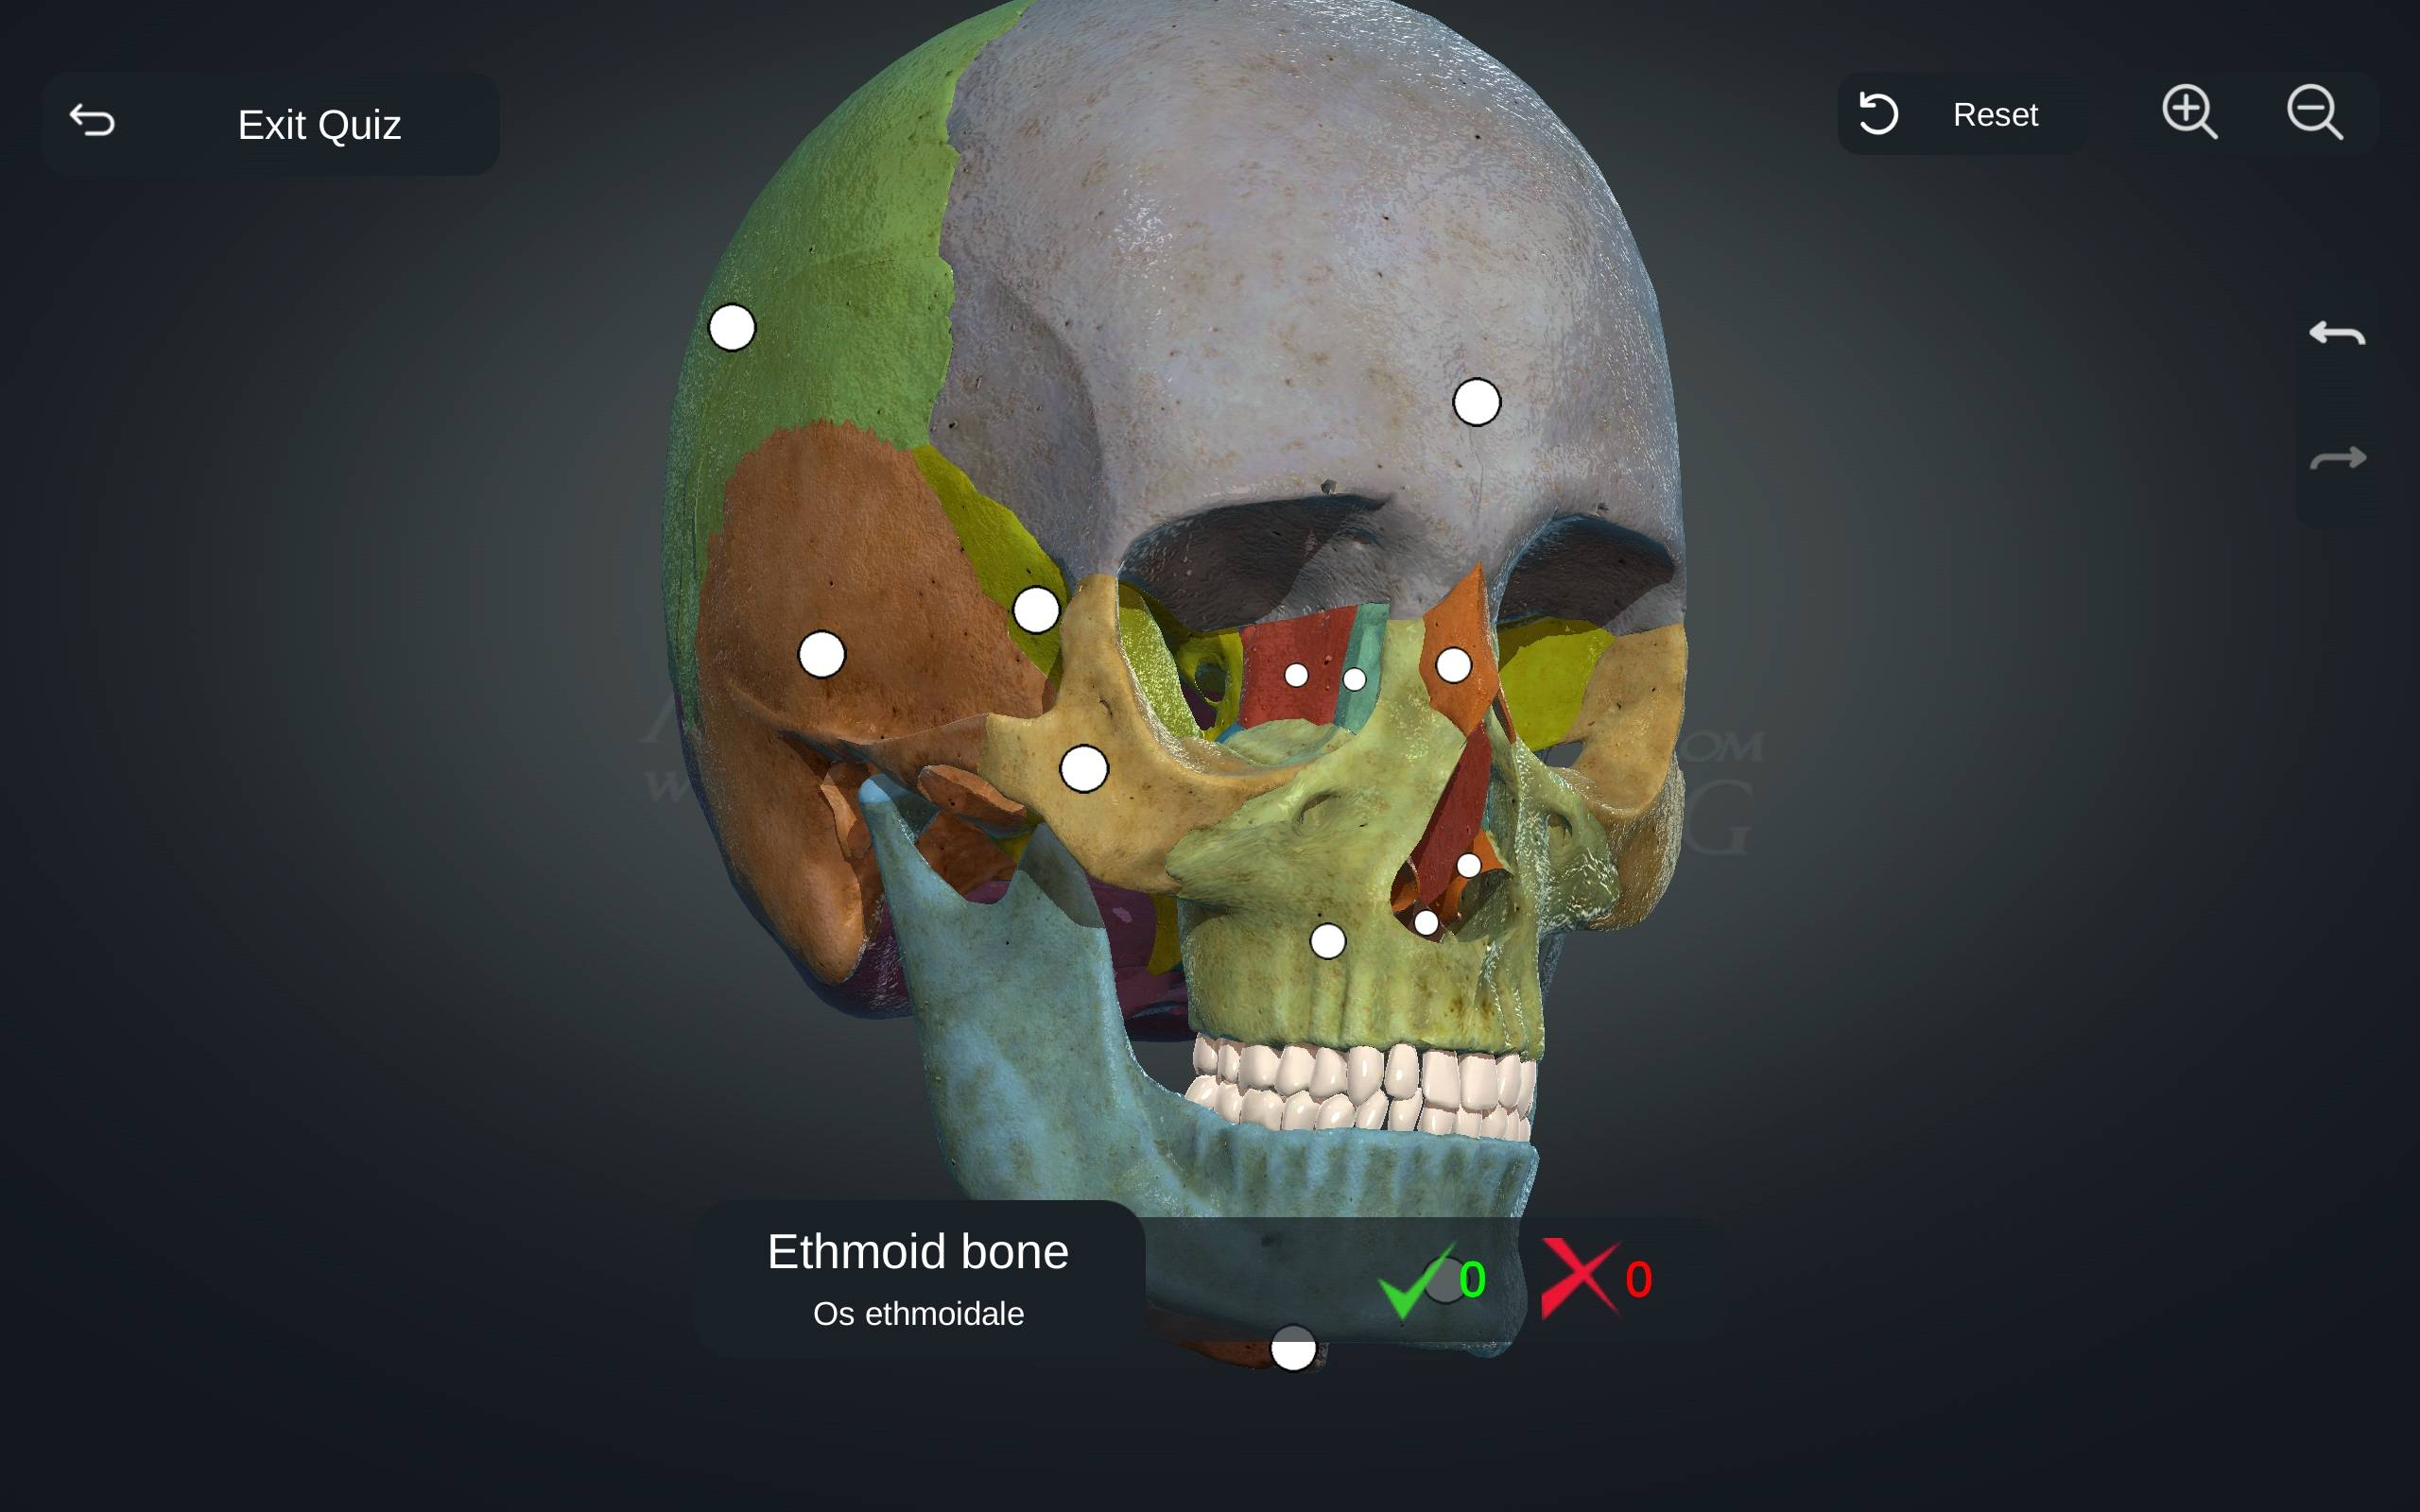
\includegraphics[width=0.8\textwidth]{Gambar/AnatomyLearning_QuizezHead.jpg}  
                        \caption [Halaman fitur \textit{Quizzes} pada aplikasi \textit{Anatomy Learning}] {Halaman fitur \textit{Quizzes} pada aplikasi \textit{Anatomy Learning}}  
                        \label{fig:QuizzesPage} 
                    \end{figure}
                                
            \item \textit{Animation}
            
                Fitur ini memungkinkan pengguna untuk memvisualisasikan mekanisme pergerakan otot dan sendi dalam bentuk video pendek. Berbeda dengan model statis pada atlas umum, fitur ini menyajikan animasi yang mendetail, sehingga pengguna dapat memahami interaksi antara sistem tulang, sendi dan otot saat terjadi gerakan tubuh tertentu, seperti fleksi, ekstensi, atau rotasi.
                
                   \begin{figure}[H] 
                        \centering  
                        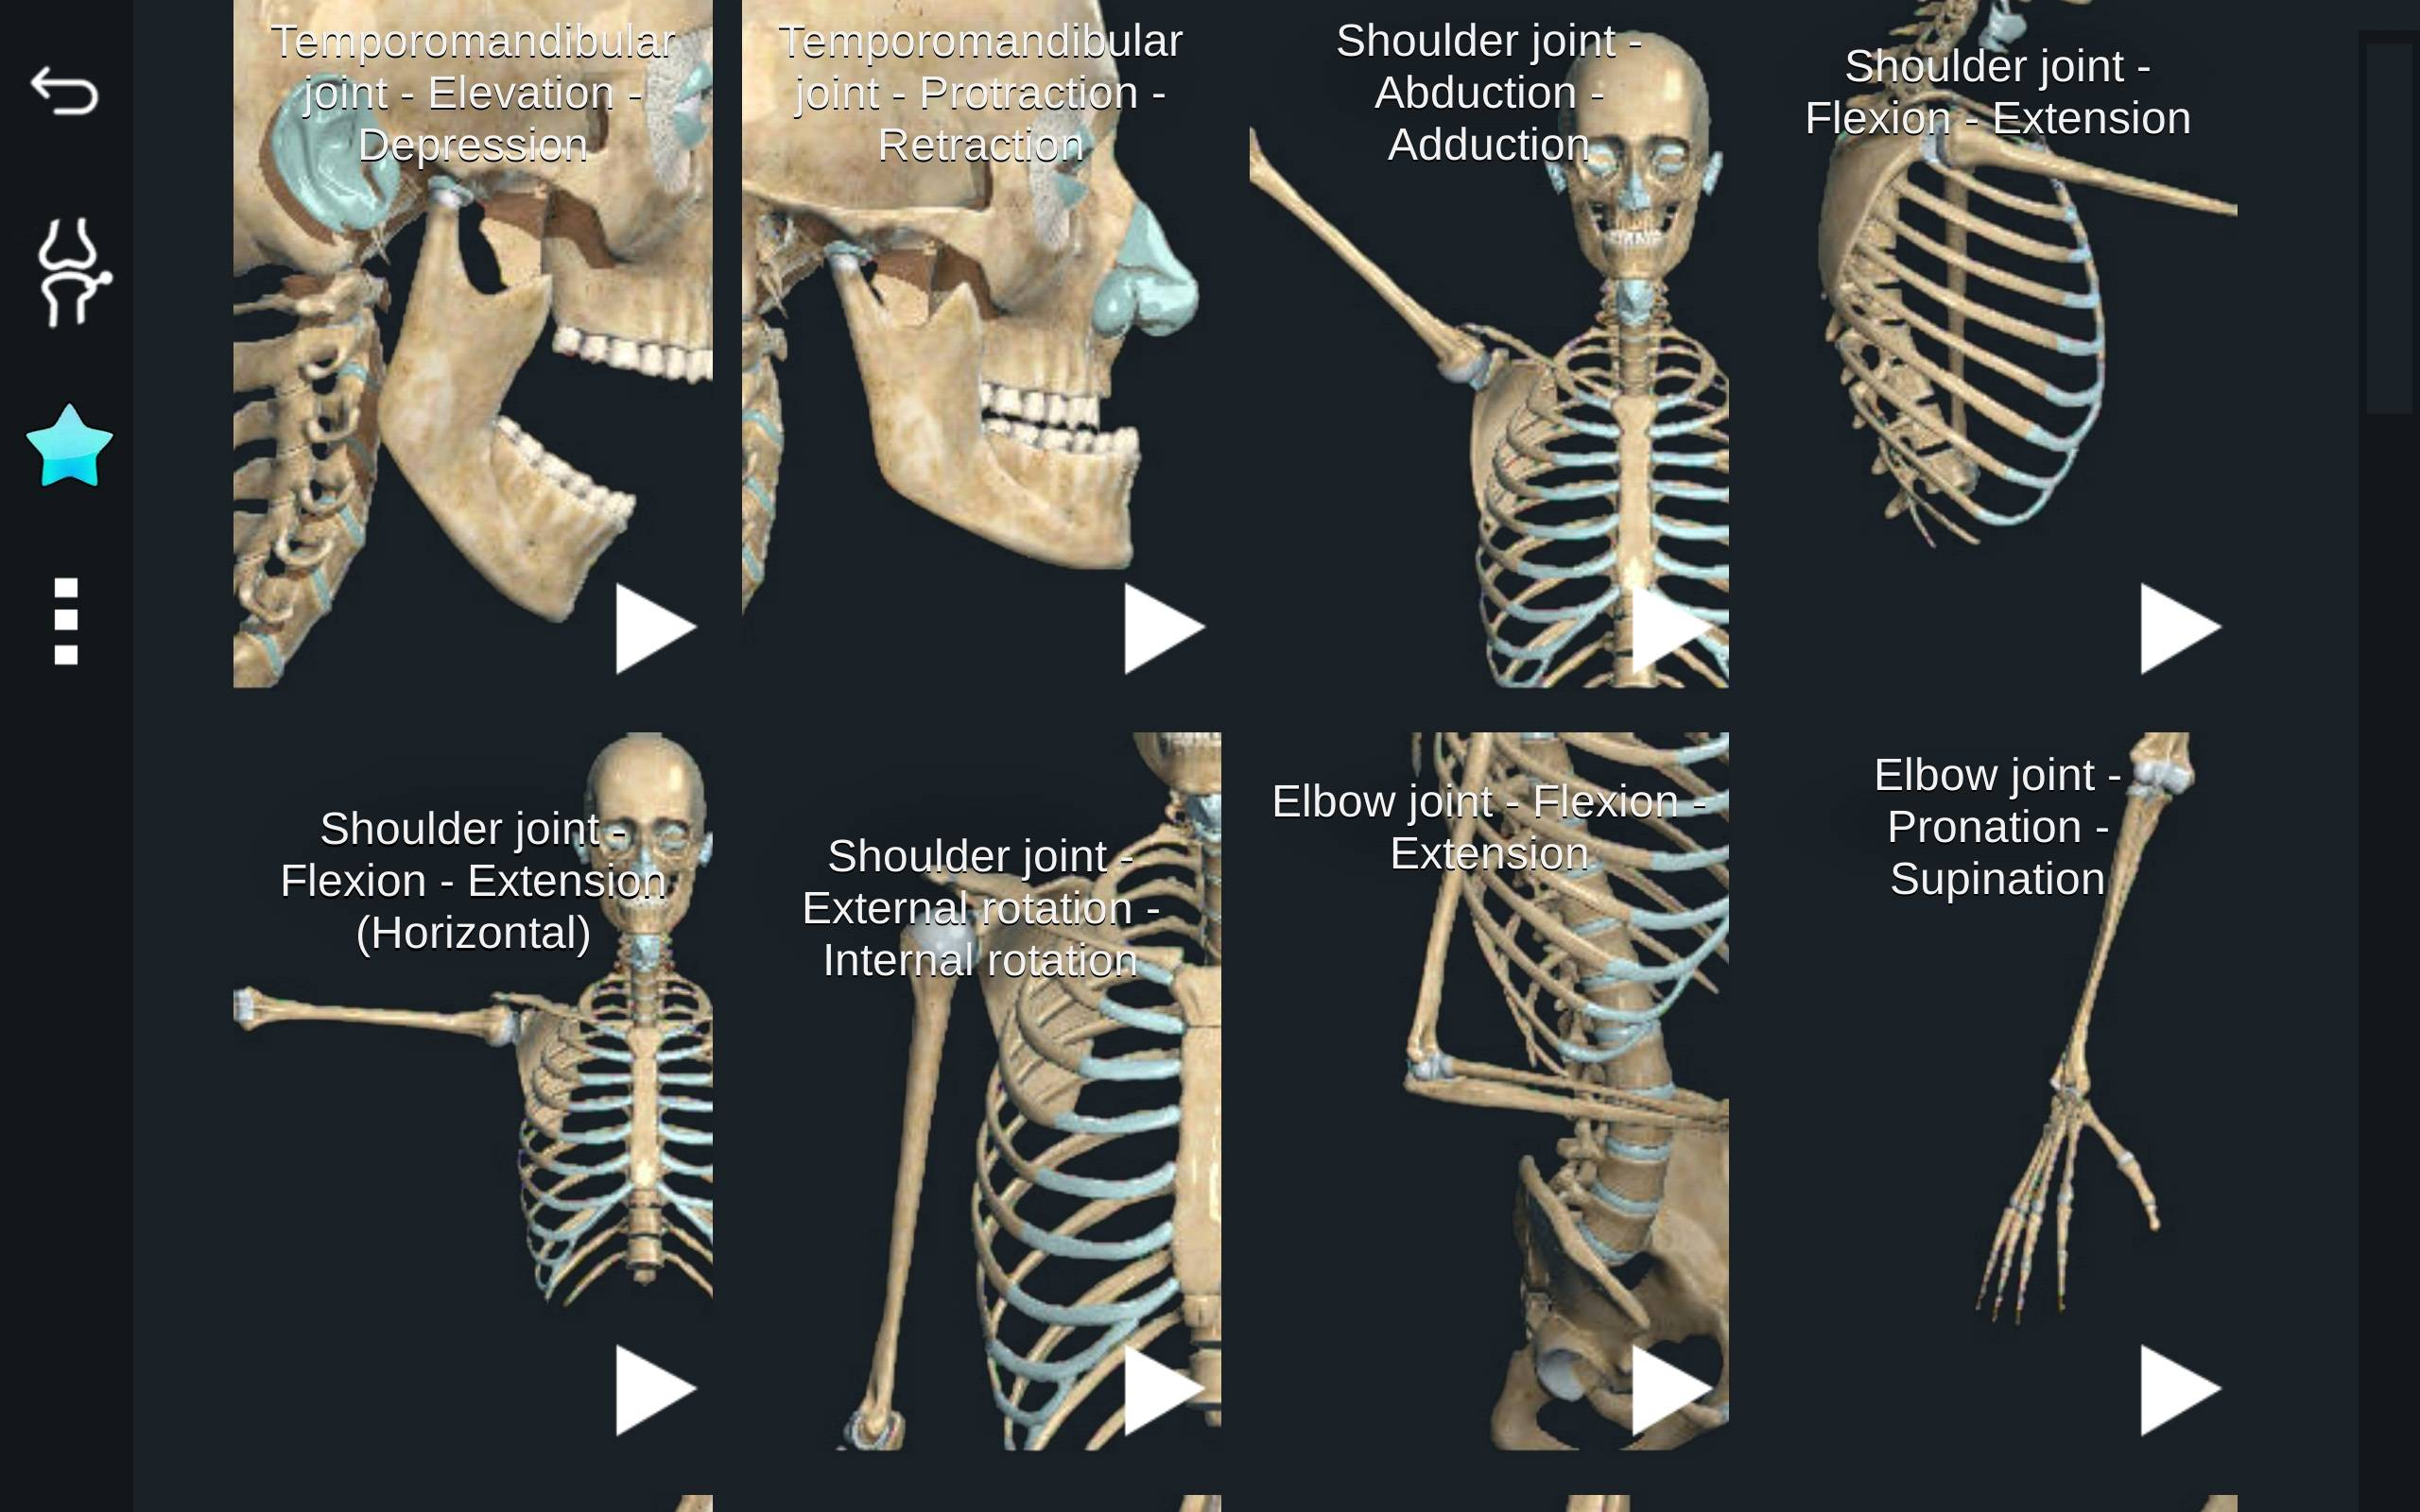
\includegraphics[width=0.8\textwidth]{Gambar/AnatomyLearning_Animaion.jpg}  
                        \caption [Halaman fitur \textit{Animation} pada aplikasi \textit{Anatomy Learning}] {Halaman fitur \textit{Animation} pada aplikasi \textit{Anatomy Learning}} 
                        \label{fig:AnimationPage} 
                    \end{figure}
                                
    
            \item \textit{Sectional Anatomy} 
    
                Fitur ini memungkinkan pengguna untuk mengatur transparansi dan visibilitas bagian tubuh yang dipilih secara selektif. Meskipun representasi visualnya menyerupai citra medis \textit{CT Scan}, fitur ini bersifat statis pada satu sudut pandang (\textit{fixed position}) untuk memberikan pemahaman mengenai struktur internal manusia.
                 \begin{figure}[H] 
                        \centering  
                        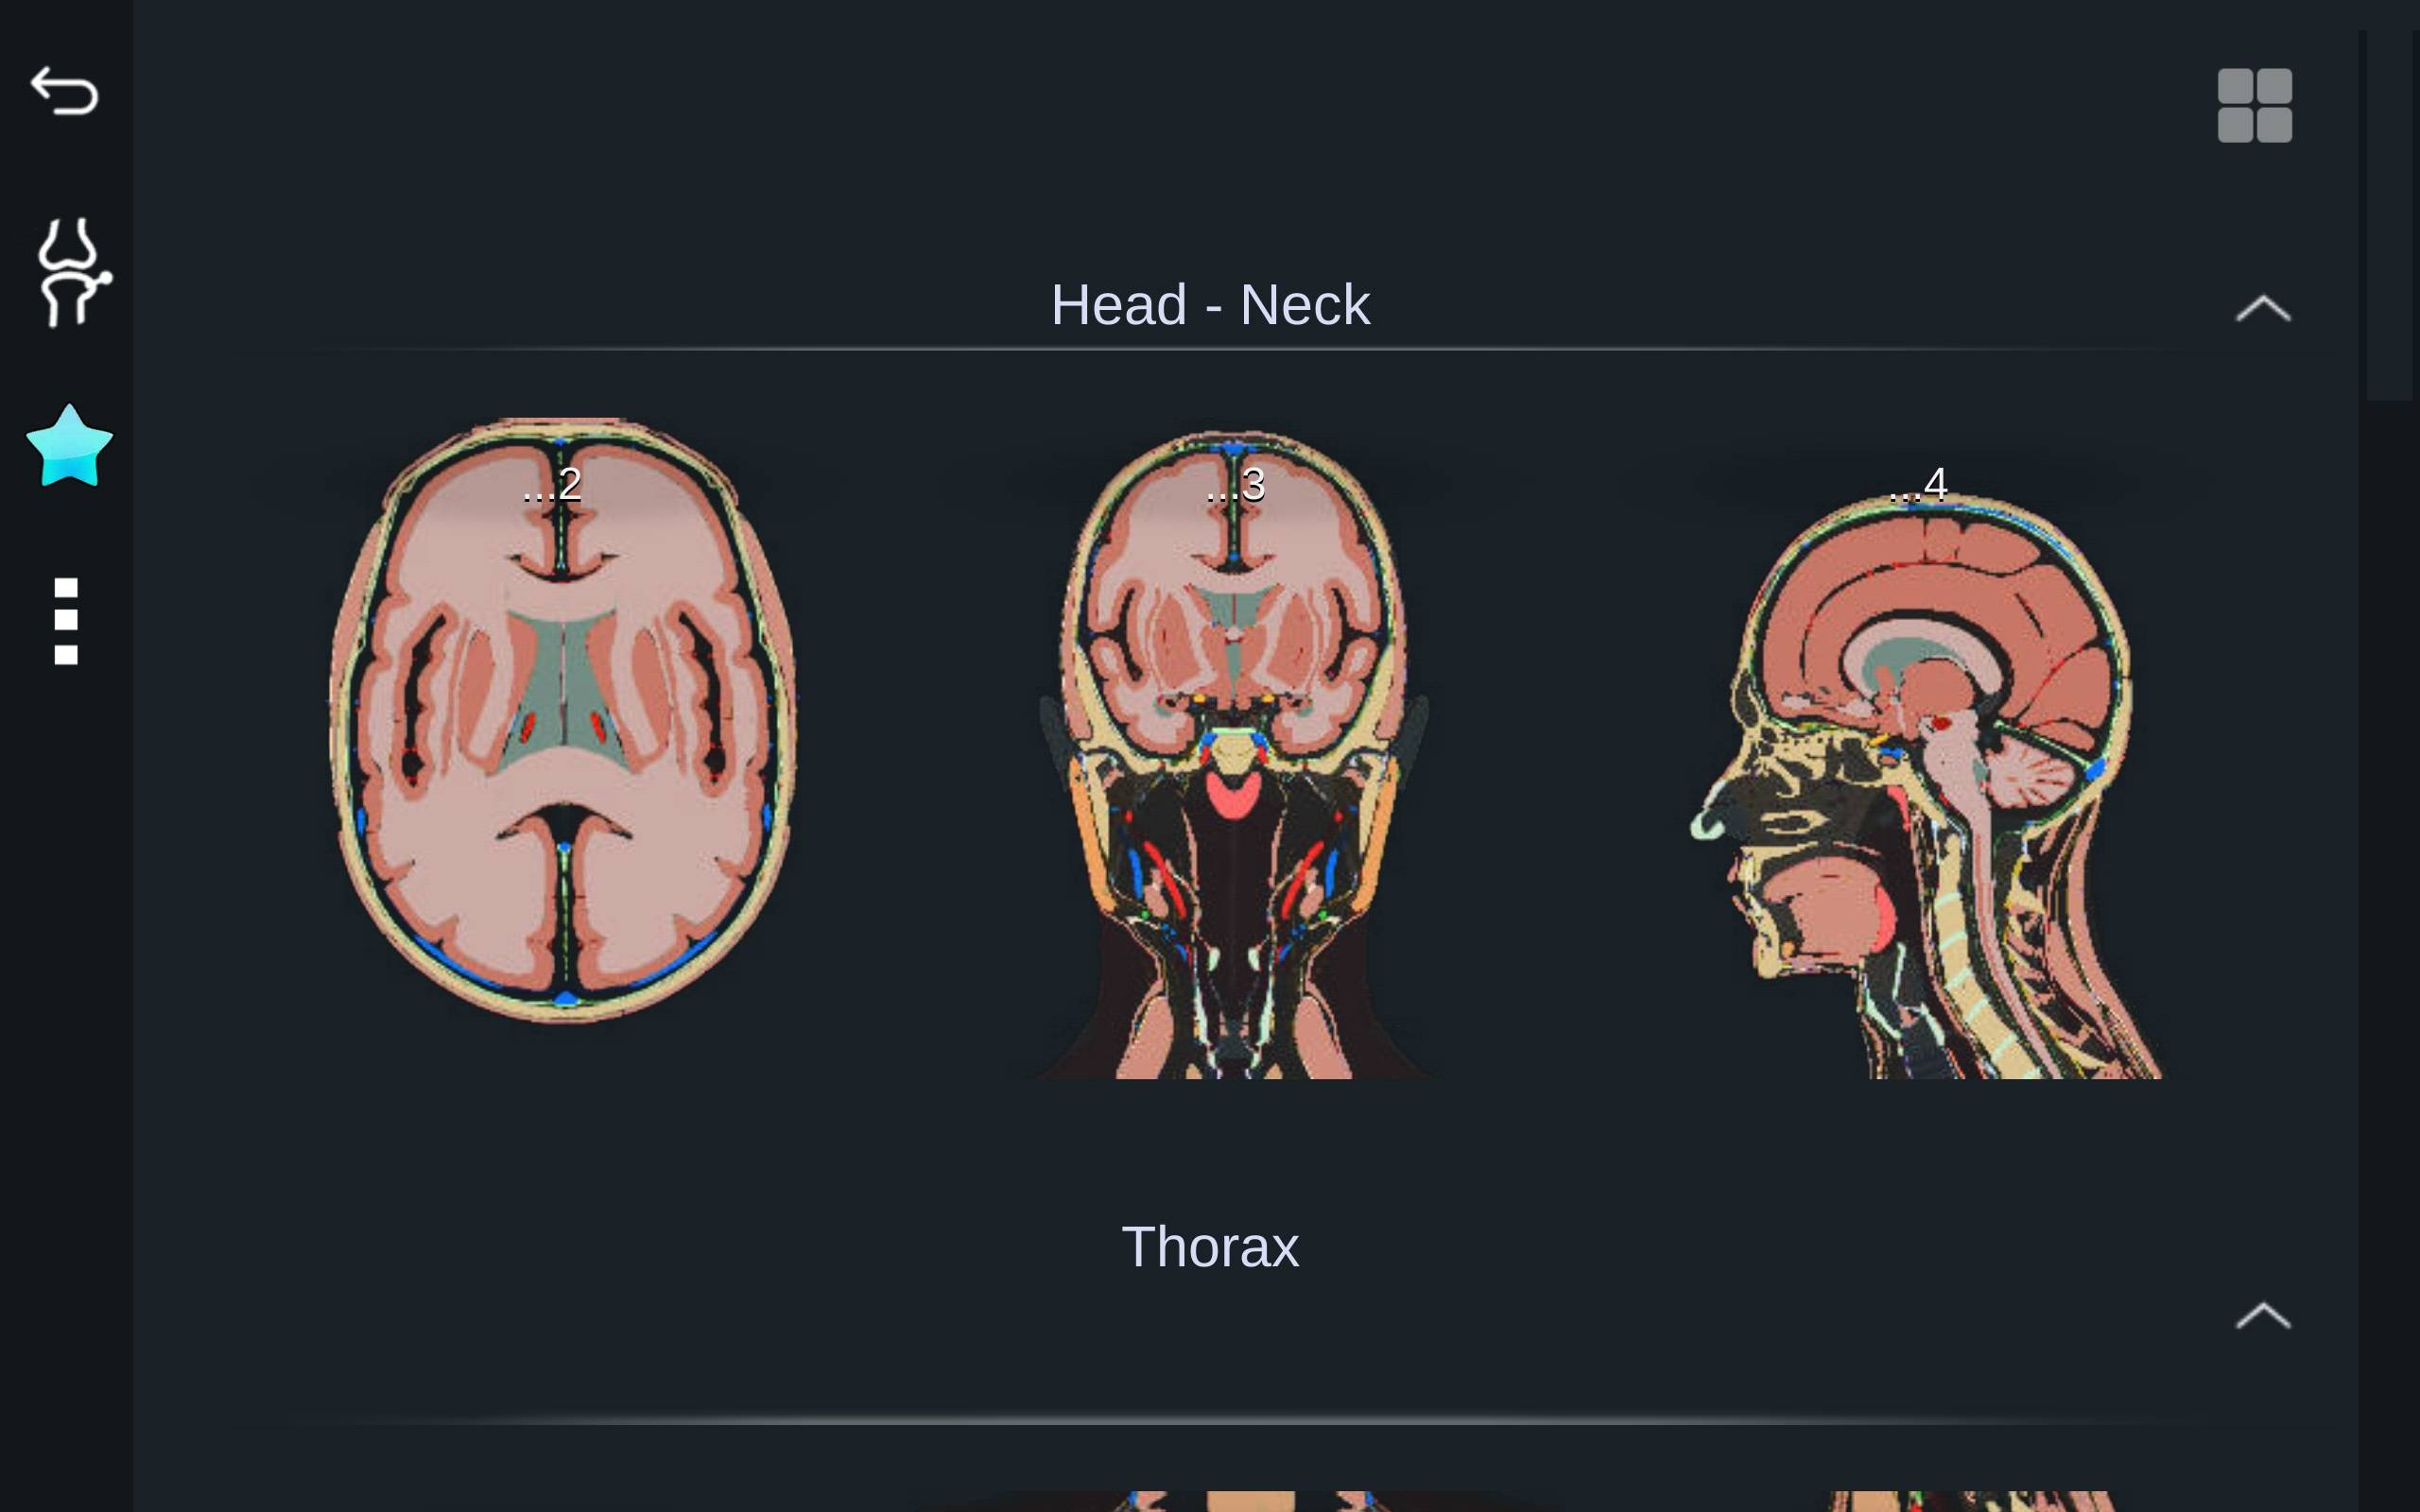
\includegraphics[width=0.8\textwidth]{Gambar/AnatomyLearning_Xray.jpg}  
                        \caption [Halaman fitur \textit{Sectional Anatomy} pada aplikasi \textit{Anatomy Learning}] {Halaman fitur \textit{Sectional Anatomy} pada aplikasi \textit{Anatomy Learning}} 
                        \label{fig:AnimationPage} 
                    \end{figure}
                                
    	      \end{enumerate}



     \subsection{\textit{Anatomy 3D Atlas}\footnote{Catfish Animation Studio, \textit{Anatomy 3D Atlas}, diunduh dari \url{https://play.google.com/store/apps/details?id=com.catfishanimationstudio.MuscularSystemLite} pada 10 Maret 2026 dengan versi 7.0.6 dan \textit{last update} pada 17 Januari 2026.}}
    
            \textit{Anatomy 3D Atlas}, yang dikembangkan oleh Catfish Animation Studio, merupakan platform edukasi medis yang dirancang untuk memfasilitasi pembelajaran anatomi manusia melalui pemodelan tiga dimensi (3D) yang interaktif. Aplikasi ini mengedepankan antarmuka pengguna yang intuitif guna mendukung eksplorasi struktur tubuh dari berbagai perspektif secara \textit{real-time}. Perangkat lunak ini ditujukan sebagai instrumen referensi bagi kalangan profesional maupun akademisi, seperti dokter, mahasiswa kedokteran, hingga praktisi kesehatan lainnya yang memerlukan pemahaman mendalam mengenai morfologi tubuh manusia.\footnote{\url{https://anatomy3datlas.com/} diakses pada 27 April 2026}

            Fitur utama pada aplikasi ini adalah atlas anatomi di mana anatomi manusia diklasifikasikan ke dalam empat kategori utama, yang kemudian dibagi menjadi sub-kategori lebih spesifik:
            \begin{itemize}
                \item \textit{Head} (Bagian Kepala)
                    \begin{itemize}
                        \item \textit{Musculoskeletal System} (Sistem Otot dan Rangka)
                        \item \textit{Cardiovascular System} (Sistem Kardiovaskular)
                        \item \textit{Nervous System} (Sistem Saraf)
                        \item \textit{Lymphatic System} (Sistem Limfatik)
                        \item \textit{Sense Organs} (Panca Indra)
                        \item \textit{All Systems} (Semua Sistem)
                    \end{itemize}
                    
                \item \textit{Trunk} (Batang Tubuh)
                    \begin{itemize}
                        \item \textit{Musculoskeletal System} (Sistem Otot dan Rangka)
                        \item \textit{Cardiovascular System} (Sistem Kardiovaskular)
                        \item \textit{Nervous System} (Sistem Saraf)
                        \item \textit{Respiratory System} (Sistem Pernapasan)
                        \item \textit{Digestive System} (Sistem Pencernaan)
                        \item \textit{Urogenital System} (Sistem Urogenital)
                        \item \textit{Lymphatic System} (Sistem Limfatik)
                        \item \textit{All Systems} (Semua Sistem)
                    \end{itemize}
                    \begin{figure}[H] 
                        \centering  
                        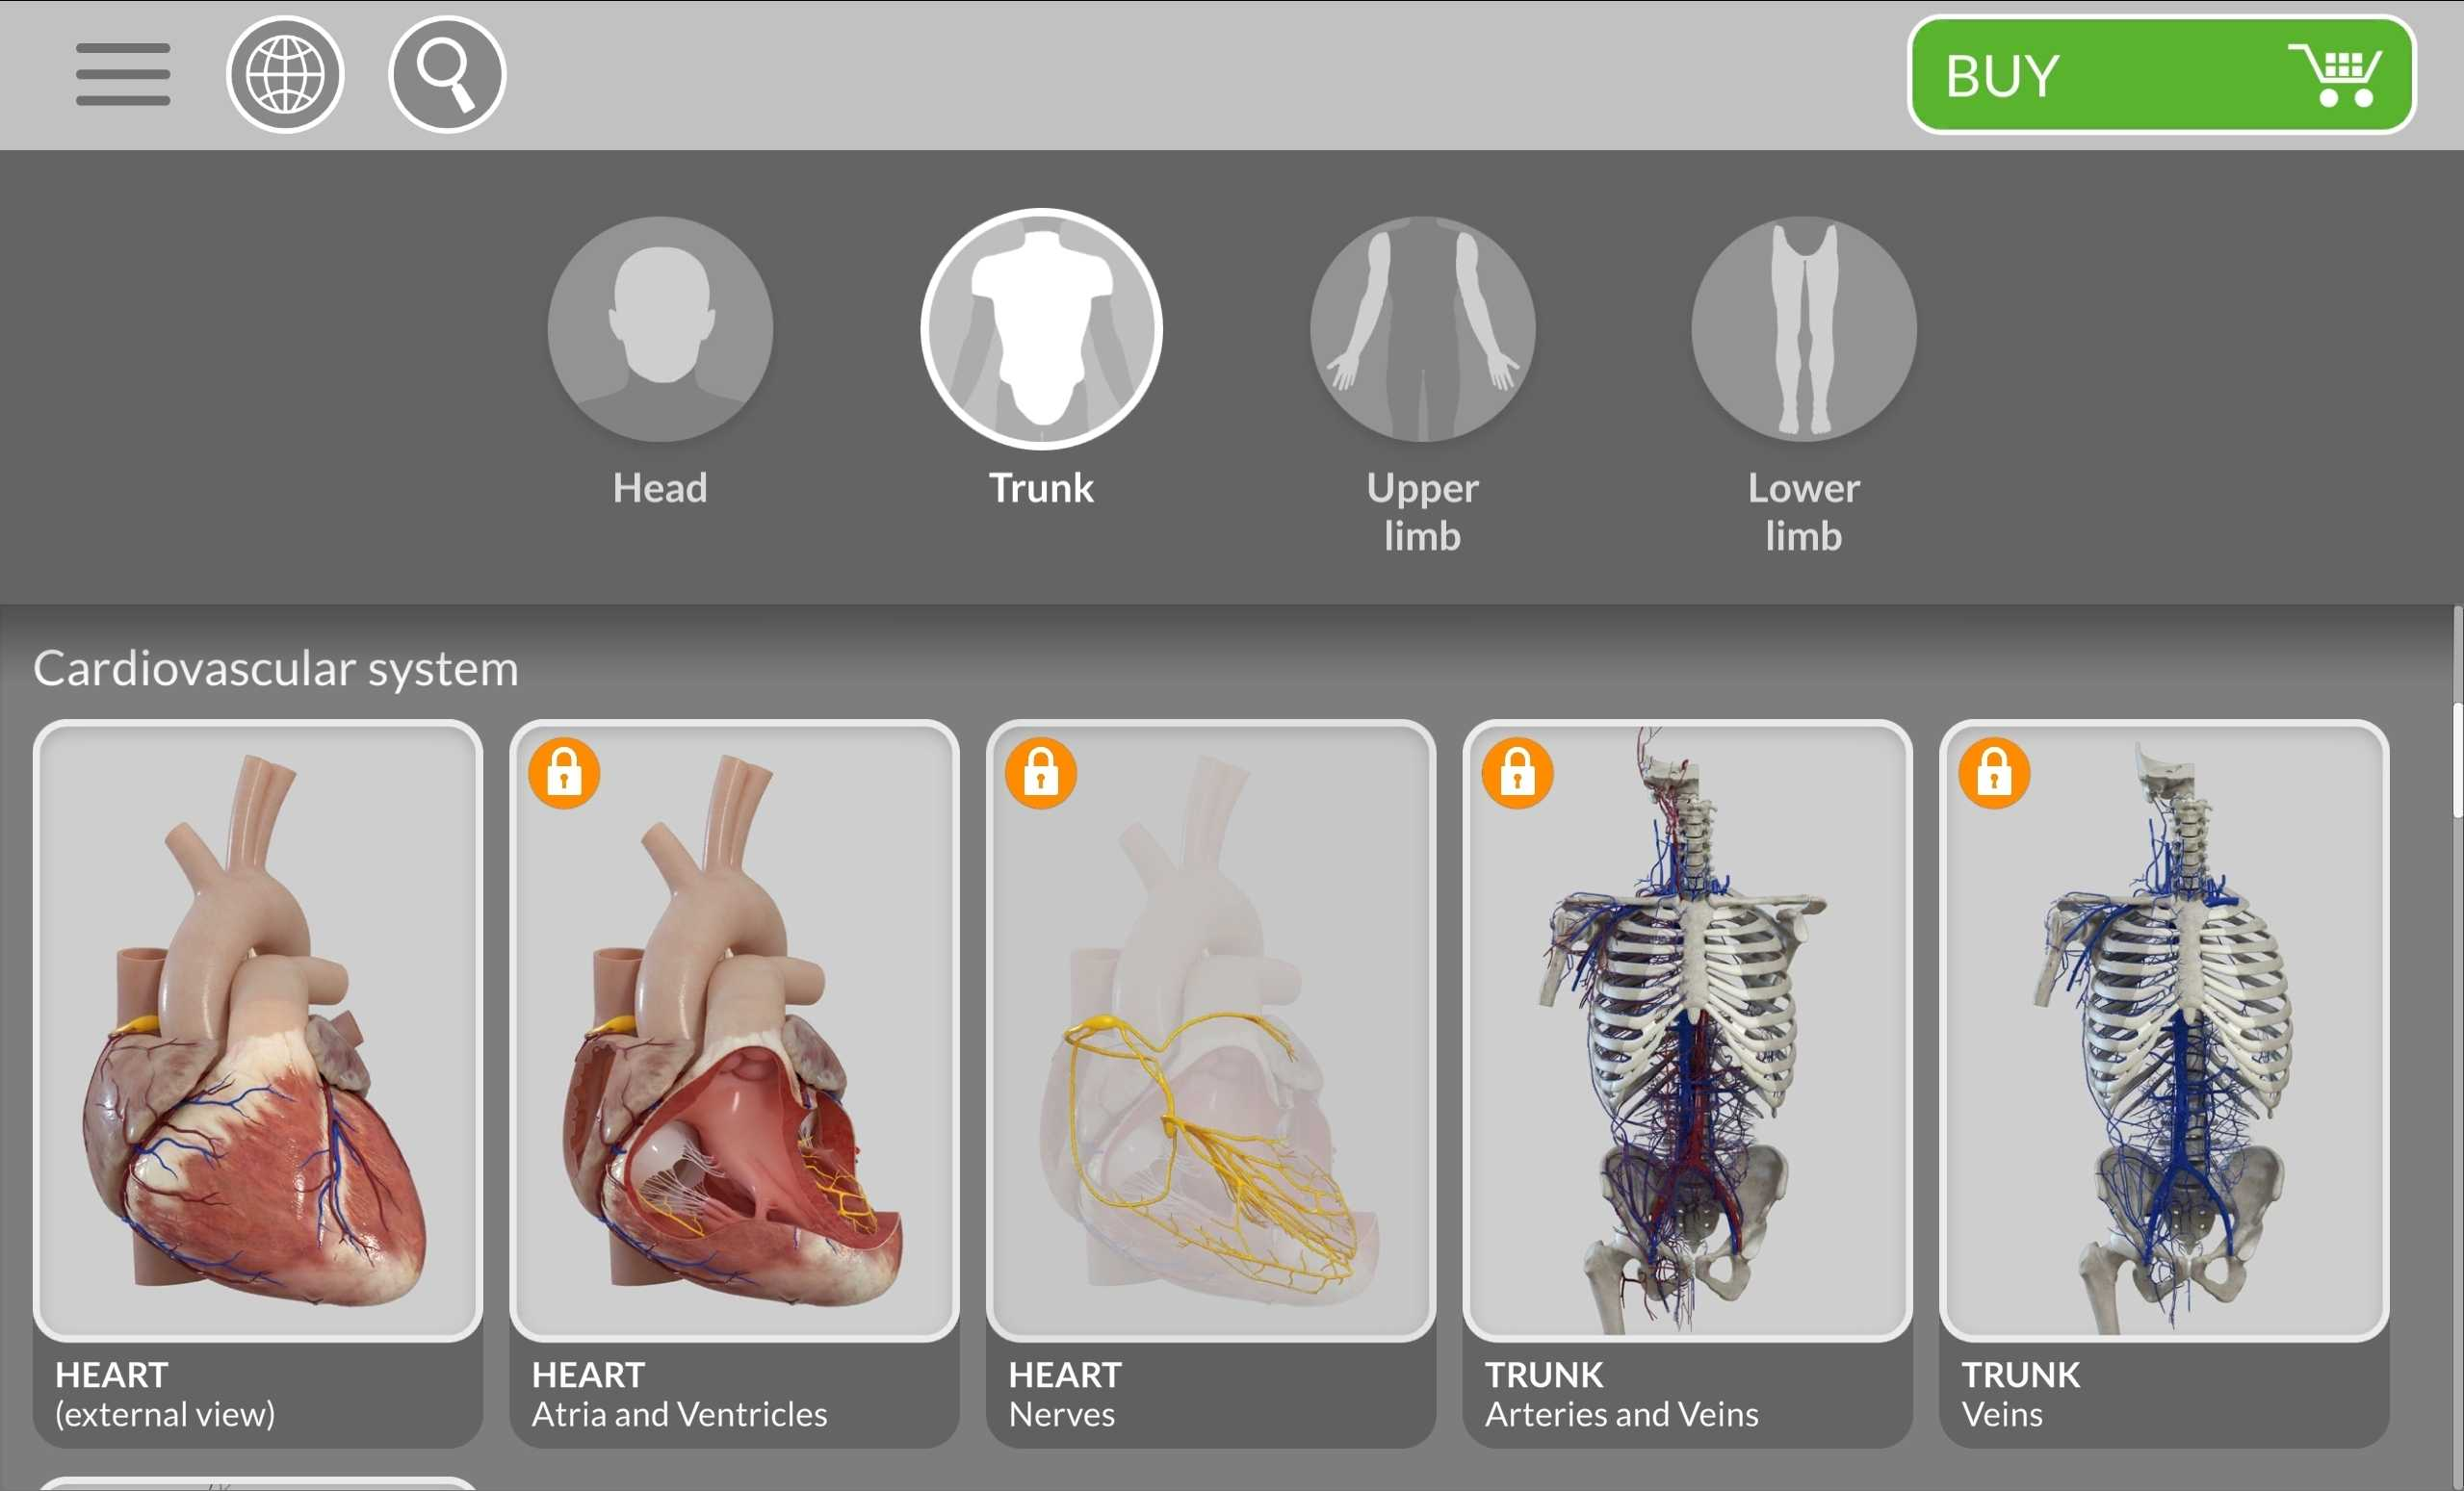
\includegraphics[width=0.8\textwidth]{Gambar/Anatomy3DAtlas_Cardiovaskular.jpg}
                        \caption [Halaman awal \textit{Trunk} bagian \textit{Cariovascular} pada aplikasi \textit{Anatomy 3D Atlas}] {Halaman awal \textit{Trunk} bagian \textit{Cariovascular} pada aplikasi \textit{Anatomy 3D Atlas}} 
                        \label{fig:Anatomy3DTrunkCardiovascular} 
                    \end{figure}
                    
                \item \textit{Upper Limb} (Anggota Gerak Atas)
                    \begin{itemize}
                        \item \textit{Musculoskeletal System} (Sistem Otot dan Rangka)
                        \item \textit{Cardiovascular System} (Sistem Kardiovaskular)
                        \item \textit{Nervous System} (Sistem Saraf)
                        \item \textit{Lymphatic System} (Sistem Limfatik)
                        \item \textit{All Systems} (Semua Sistem)
                    \end{itemize}
                    
                \item \textit{Lower Limb} (Anggota Gerak Bawah)
                    \begin{itemize}
                        \item \textit{Musculoskeletal System} (Sistem Otot dan Rangka)
                        \item \textit{Cardiovascular System} (Sistem Kardiovaskular)
                        \item \textit{Nervous System} (Sistem Saraf)
                        \item \textit{Lymphatic System} (Sistem Limfatik)
                        \item \textit{All Systems} (Semua Sistem)
                    \end{itemize}
            \end{itemize}
            \begin{figure}[H] 
                        \centering  
                        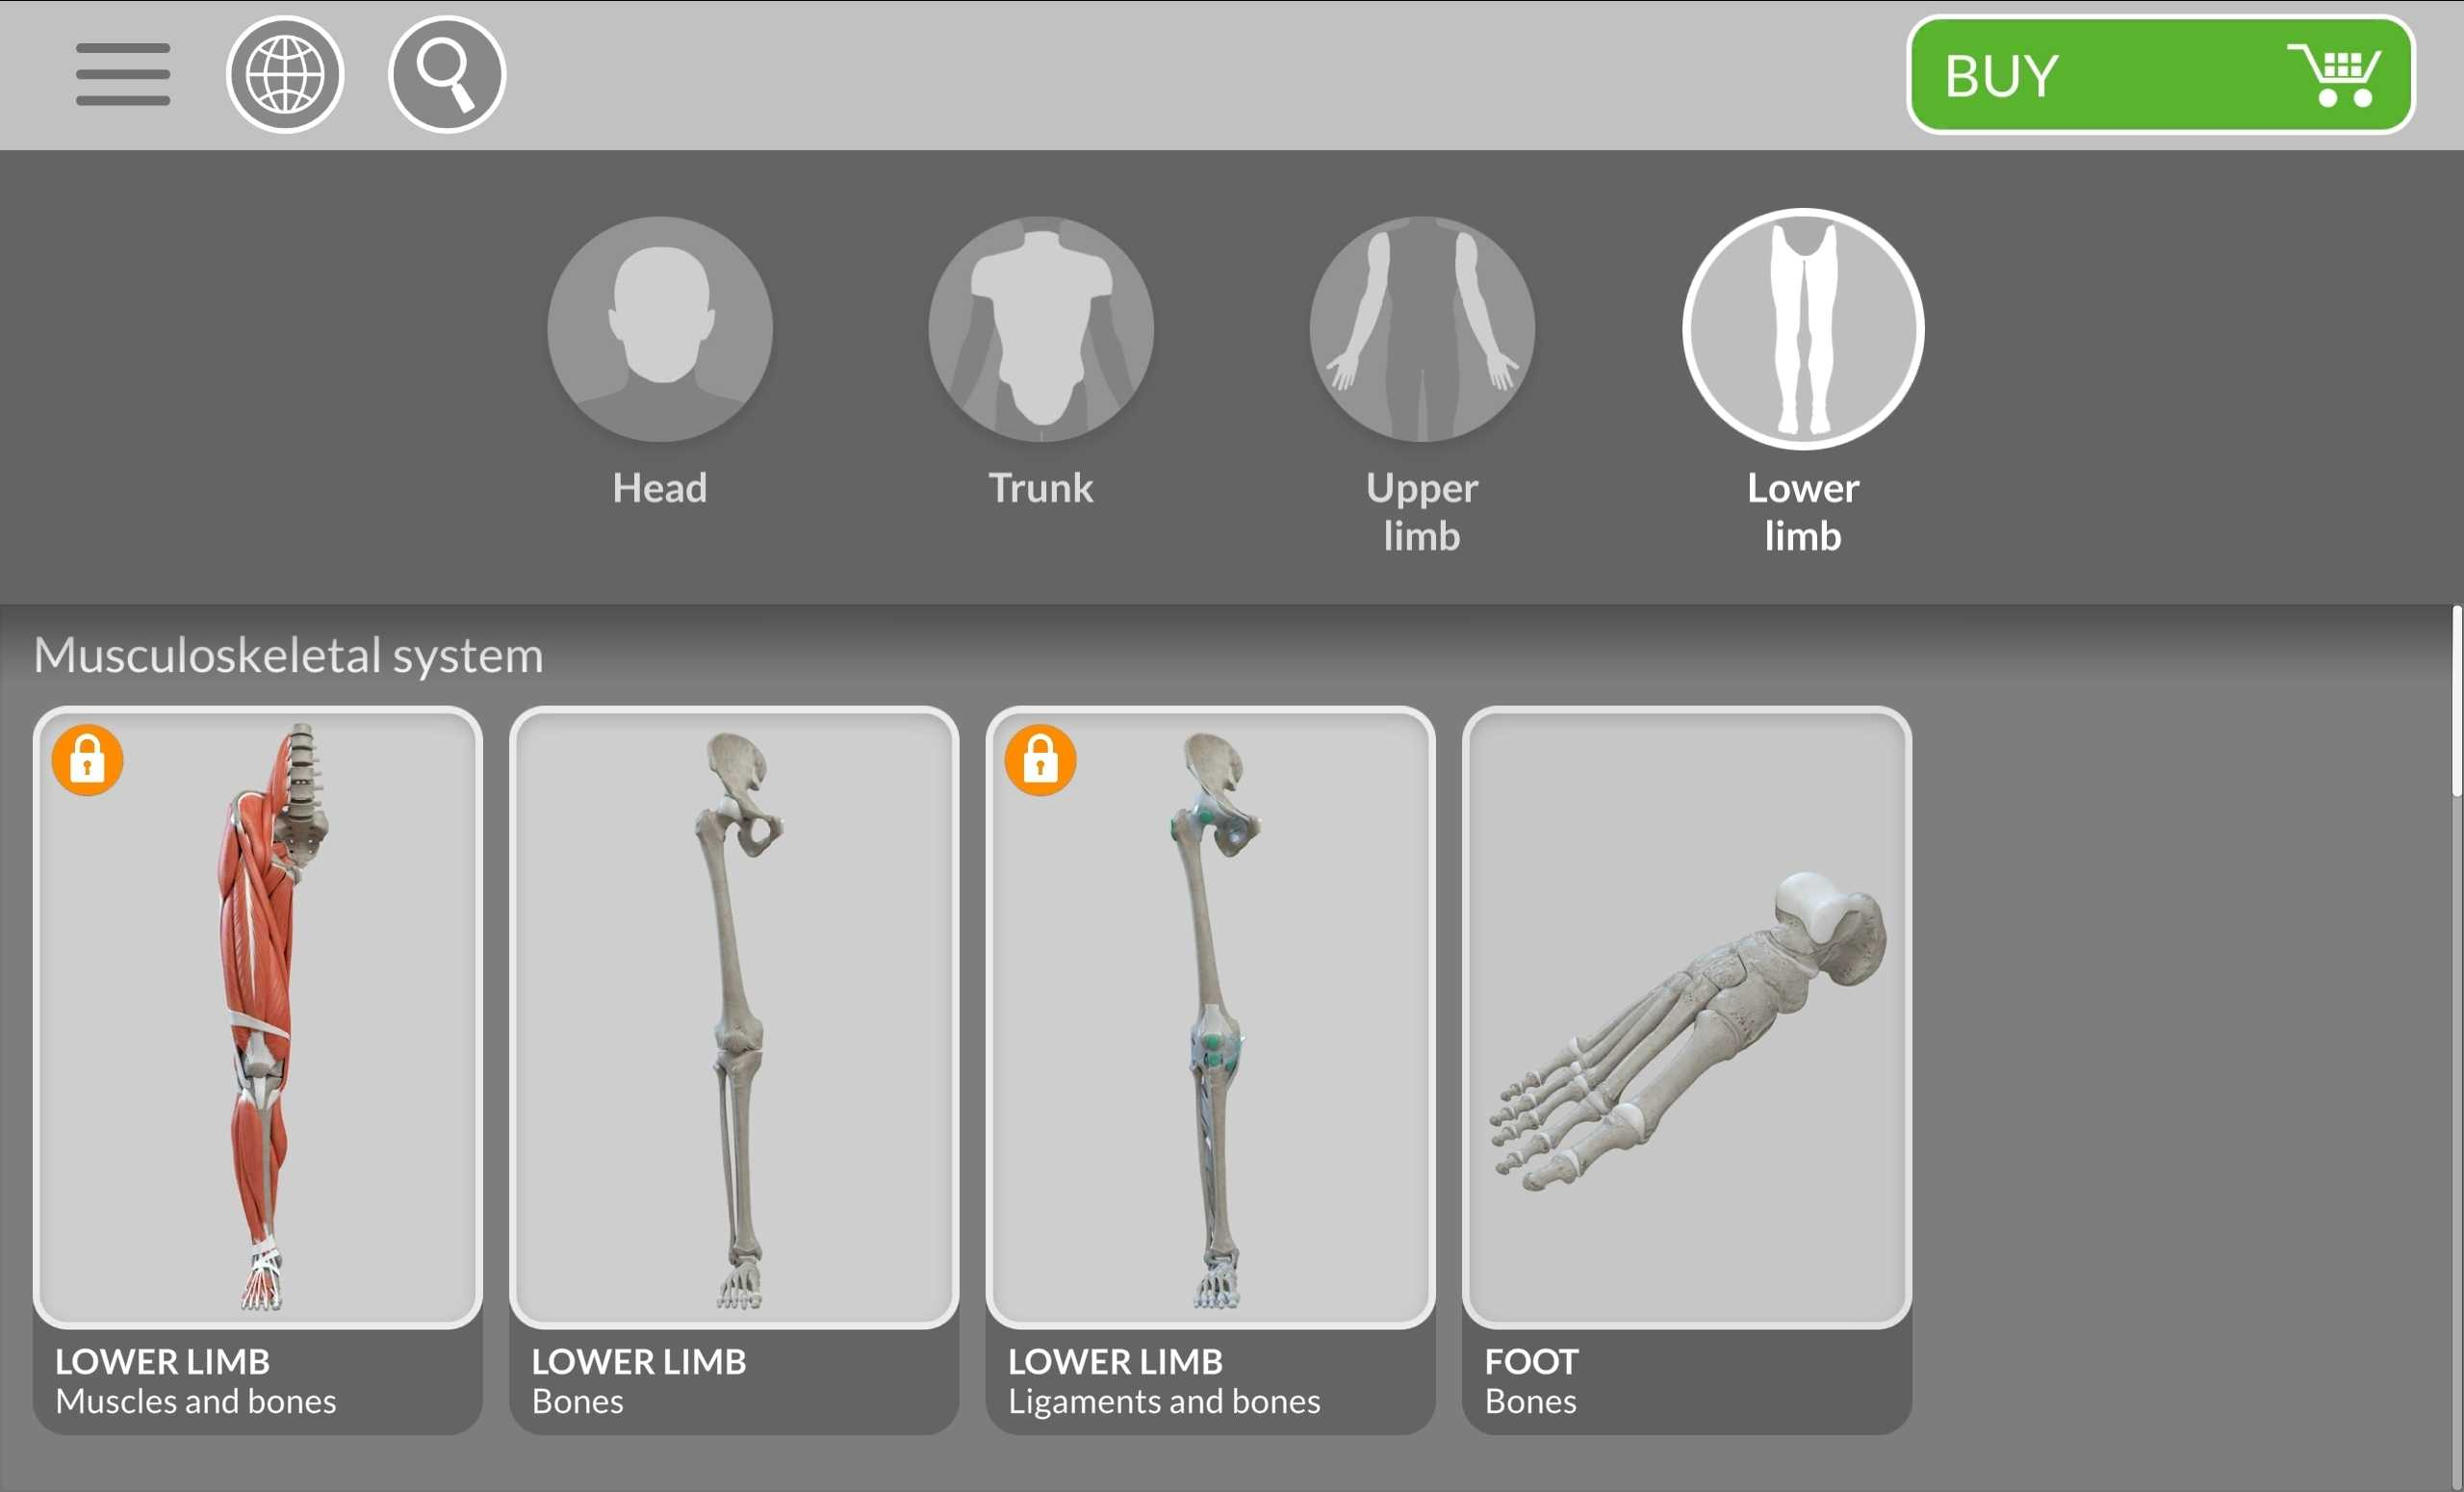
\includegraphics[width=0.8\textwidth]{Gambar/Anatomy3DAtlas_MusculoskeletalSystemLower.jpg}
                        \caption [Halaman awal \textit{Lower Limb} bagian \textit{Musculoskeletal} pada aplikasi \textit{Anatomy 3D Atlas}] {Halaman awal \textit{Lower Limb} bagian \textit{Musculoskeletal} pada aplikasi \textit{Anatomy 3D Atlas}} 
                        \label{fig:Anatomy3DTrunkCardiovascular} 
            \end{figure}
            
        \subsection {Perbandingan Kedua Aplikasi}
        \begin{itemize}
            \item \textit{Anatomy Learning} 
                \begin{itemize}
                    \item Memiliki fitur \textit{Quizzes} untuk membantu dalam pemahaman anatomi secara aktif.
                    \item Memiliki fitur \textit{Animation} untuk membantu memahami biomekanika atau apa yang terjadi pada tubuh manusia saat bergerak.
                    \item Fokus pada penjelasan fungsi (\textit{physiology}) selain bentuk fisik.
                \end{itemize}
                
            \item \textit{Anatomy 3D Atlas} 
                \begin{itemize}
                    \item Menyediakan detail struktur yang lebih kompleks dan mendalam untuk keperluan profesional/medis.
                    \item Fokus utama pada penamaan ilmiah (\textit{nomenclature}).
                    \item Tidak memiliki fitur \textit{Quizzes} lebih berfokus sebagai referensi visual cepat.
                    \item Tidak memiliki fitur \textit{Animation} objek cenderung statis dalam posisi anatomi standar.
                \end{itemize}
        \end{itemize}
        
    \section{Analisis Model 3D}
        Pemilihan aset model 3D yang digunakan sebagai basis data visual dalam sistem ini harus memperhatikan aspek lisensi yang menyertainya. Lisensi merupakan instrumen hukum yang mengatur batasan penggunaan suatu karya digital, memberikan perlindungan terhadap hak cipta pencipta, serta mencegah penggunaan aset secara tidak bertanggung jawab atau tanpa izin. 
        
        Dalam proses akuisisi aset, analisis lisensi menjadi krusial karena beberapa model memerlukan kompensasi finansial (berbayar) atau kewajiban atribusi tertentu. Oleh karena itu, pemilihan model pada penelitian ini difokuskan pada aset yang memiliki ketentuan penggunaan yang selaras dengan tujuan pengembangan sistem, baik dari segi legalitas modifikasi maupun distribusi di dalam perangkat lunak berbasis web.
 
        \subsection{Splanchnology \footnote{\url{https://sketchfab.com/3d-models/splanchnology-5cfafb312f504815aa3fec55735607a6} diakses pada Maret 2026}}
            Berikut adalah detail karakteristik teknis dan ketentuan lisensi yang menyertai aset tersebut:
                    
            \begin{enumerate}
                \item \textbf{Karakteristik Geometri dan Segmentasi:}
                Aset ini merupakan pengembangan versi kedua dari basis data visual ``BodyParts3D'' yang saat ini sudah tidak tersedia secara publik. Model ini menyajikan struktur organ internal secara komprehensif, mencakup organ utama seperti paru-paru, jantung, hati, dan lambung. Keunggulan teknis aset ini terletak pada segmentasi objek yang detail, di mana setiap organ direpresentasikan sebagai \textit{mesh} terpisah. Struktur ini memungkinkan sistem untuk mengimplementasikan fitur interaktif seperti isolasi organ tunggal serta pengaturan transparansi per lapisan secara independen.
            
                \item \textbf{Lisensi:}
                Aset ini didistribusikan secara gratis di bawah lisensi \textit{Creative Commons Attribution} (CC BY-SA 4.0), yang memberikan kepastian hukum melalui izin penggunaan terbuka dengan kewajiban atribusi. Ketentuan lisensi ini memberikan hak adaptasi bagi pengembang untuk melakukan modifikasi teknis, seperti optimasi jumlah poligon (\textit{polygon count}) guna efisiensi performa pada \textit{web browser}. Sebagai bentuk kepatuhan terhadap kewajiban lisensi, pemberian kredit dilakukan dengan mencantumkan identitas kreator dan tautan sumber aset pada menu \textit{About} atau \textit{Credit} di dalam aplikasi. Penggunaan lisensi ini memberikan fleksibilitas tinggi karena tidak membatasi penggunaan untuk tujuan komersial maupun non-komersial.

                \item \textbf{Perbandingan dengan Aplikasi Referensi:}
                Jika dibandingkan dengan aset yang digunakan pada aplikasi \textit{Anatomy Learning} dan \textit{Anatomy 3D Atlas}, model \textit{Splanchnology} ini memiliki karakteristik yang spesifik dari segi struktur dan fleksibilitas pengembangan:
                \begin{itemize}
                    \item \textit{Anatomy Learning}: Jika \textit{Anatomy Learning} mengandalkan model dengan animasi terintegrasi untuk mendemonstrasikan mekanisme fisiologi dan artikulasi sendi yang kompleks, model \textit{Splanchnology} lebih bersifat statis. Namun, karakteristik statis ini memberikan efisiensi yang lebih baik dan fokus pada detail morfologi organ internal tanpa beban data animasi yang berat.
                    
                    \item \textit{Anatomy 3D Atlas}: Aplikasi \textit{Anatomy 3D Atlas} menggunakan model yang sudah ``terkunci'' dan sangat berat karena detailnya yang terlalu tinggi, sehingga sulit diubah. Sebaliknya, model \textit{Splanchnology} lebih fleksibel karena bisa disederhanakan detail modelnya agar aplikasi tidak lambat saat dibuka di \textit{browser}.

                \end{itemize}
            \end{enumerate}
            
            
      
        \subsection{Complete Human Male Anatomy\footnote{\url{https://www.fab.com/listings/11bd315b-74a9-4960-8849-294290c979a8} diakses pada Mei 2026}}
        Berikut adalah detail mengenai karakteristik teknis dan ketentuan lisensi untuk model anatomi lengkap tersebut:
        
             \begin{enumerate}
                \item \textbf{Karakteristik Geometri dan Detail Visual:}
                Model ini menyajikan representasi anatomi pria yang mendalam, mencakup struktur kerangka (\textit{skeleton}), sistem otot (\textit{muscles}), hingga organ dalam yang ditempatkan secara presisi dalam satu kesatuan. Keunggulan utama aset ini adalah kualitas visual yang sangat tinggi dengan detail tekstur yang realistis, menjadikannya basis data visual yang ideal untuk fitur identifikasi organ. 
            
               \item \textbf{Lisensi:}
                Aset ini diperoleh secara berbayar melalui \textit{Fab Standard License} dari Epic Games serta memiliki lisensi \textit{Creative Commons Attribution} (CC BY 4.0). Lisensi ini memberikan hak penggunaan profesional yang memungkinkan pengembang untuk menggunakan, memodifikasi, dan mengintegrasikan aset ke dalam perangkat lunak secara permanen. Berbeda dengan lisensi terbuka, \textit{Fab Standard License} tidak mewajibkan pemberian atribusi kepada pencipta asli, namun secara ketat melarang distribusi ulang aset mentah. Oleh karena itu, sistem dirancang dengan mekanisme proteksi di mana pengguna hanya dapat berinteraksi dengan model melalui antarmuka aplikasi tanpa dapat mengakses atau mengunduh file sumber asli, guna mematuhi batasan hukum dan melindungi hak kekayaan intelektual yang telah dibeli.
                
                \item \textbf{Perbandingan dengan Aplikasi Referensi:}
                \begin{itemize}
                    \item \textit{Anatomy Learning}: Model ini memiliki tingkat detail permukaan (\textit{surface detail}) yang lebih realistis dan proporsional dibandingkan model pada \textit{Anatomy Learning} yang cenderung bersifat disederhanakan untuk kebutuhan animasi. Selain itu, tekstur pada aset ini menyajikan detail mikroskopis kulit dan serat otot yang lebih mendalam, memberikan impresi visual yang lebih mendekati struktur anatomi asli.
                    
                   \item \textit{Anatomy 3D Atlas}: Dari segi keakuratan geometri, model ini memiliki kualitas detail yang setara dengan \textit{Anatomy 3D Atlas}, namun dengan keunggulan pada aspek fleksibilitas tampilan. Jika model pada \textit{Anatomy 3D Atlas} sering kali memiliki tampilan visual yang sudah terstandarisasi dan statis, model ini memiliki keunggulan pada tekstur dan pencahayaan yang lebih alami.
                \end{itemize}
            \end{enumerate}

        \subsection{Animated Full Human Body Anatomy\footnote{\url{https://www.fab.com/listings/2a0d65fb-c7b5-4446-8fdd-80e5cbed47e0} diakses pada Mei 2026}}
        Berikut adalah detail mengenai karakteristik teknis dan ketentuan lisensi untuk model anatomi manusia animasi tersebut:

        \begin{enumerate}
            \item \textbf{Karakteristik Geometri dan Detail Visual:}
            Model ini menyediakan representasi anatomi tubuh manusia yang komprehensif dan dinamis, mencakup sistem kerangka, sistem otot, kulit, hingga organ dalam yang mendetail seperti otak, jantung, paru-paru, dan sistem pencernaan. Keunggulan utama aset ini adalah integrasi fitur animasi pada organ-organ vital (seperti jantung dan paru-paru) serta sistem peredaran darah, yang memberikan dimensi fungsional selain sekadar visual statis. Model ini dioptimalkan untuk performa tinggi dalam lingkungan \textit{Augmented Reality (AR}) dan \textit{Virtual Reality (VR)} tanpa mengorbankan akurasi anatomi. Setiap bagian organ bersifat \textit{detachable} (dapat dipisahkan), memungkinkan identifikasi dan isolasi struktur tubuh secara spesifik dalam aplikasi edukasi.

            \item \textbf{Lisensi:}
             Aset ini merupakan konten berbayar yang diakuisisi melalui \textit{Fab Standard License} dari Epic Games serta mengikuti ketentuan \textit{Creative Commons Attribution} (CC BY 4.0). Skema lisensi tersebut memberikan wewenang penggunaan profesional bagi pengembang untuk mengolah, mengubah, maupun menyematkan aset ke dalam sistem perangkat lunak secara permanen. Untuk menjamin kepatuhan hukum dan menjaga hak kekayaan intelektual, sistem ini dilengkapi dengan proteksi akses, yaitu pengguna hanya diberikan izin berinteraksi melalui antarmuka aplikasi tanpa memiliki akses langsung untuk mengunduh berkas mentah (\textit{source file}) model tersebut.
        
            \item \textbf{Perbandingan dengan Aplikasi Referensi:}
            \begin{itemize}
                \item \textit{Anatomy Learning}: Berbeda dengan model pada \textit{Anatomy Learning} yang bersifat statis, aset ini memiliki keunggulan pada aspek animasi fungsional (seperti detak jantung dan pernapasan paru-paru) yang lebih hidup.
                
                \item \textit{Anatomy 3D Atlas}: Dari sisi teknis, model ini menawarkan fleksibilitas lebih tinggi untuk platform interaktif (AR/VR) karena optimasi. Sementara \textit{Anatomy 3D Atlas} unggul dalam visualisasi atlas statis yang baku, model ini memberikan nilai tambah berupa visualisasi proses fisiologis melalui animasi, menjadikannya referensi yang lebih unggul untuk menjelaskan mekanisme kerja organ secara \textit{real-time}.
            \end{itemize}
        \end{enumerate}
        
\section{Analisis Perangkat Lunak yang Akan Dikembangkan}
    \subsection{Pemilihan Model}
    Proses pemilihan aset model 3D merupakan tahapan krusial dalam pengembangan aplikasi visualisasi anatomi ini. Keputusan pemilihan didasarkan pada keseimbangan antara akurasi medis, fleksibilitas pengembangan teknis, dan kepatuhan terhadap lisensi penggunaan. Berdasarkan pertimbangan tersebut, model \textit{Splanchnology} dipilih. 



